\clearpage
\section{Results and interpretation}

At the time of writing this thesis, the search presented here is in the final stages of approval by a CMS committee at CERN. Therefore, instead of unblinding the full Run 2 luminosity, 10\% of the luminosity is unblinded in the following section. The results section will be divided into two parts. Section~\ref{sec:expected-limits} presents the expected limits of the full Run 2 luminosity without observed data, which allows for a comparison of the sensitivity of this search to previous searches. Section~\ref{sec:unblinded-limits} presents the observed and predicted counts for the 10\% Run 2 luminosity alongside the calculated limits.

The results are interpreted in terms of the compressed Higgsino simplified model described in Section~\ref{sec:search-introduction}. The LSP is dominated by the Higgsino component, meaning that the Higgsino mass parameter $\mu$ is much smaller than the magnitude of the bino and wino mass parameters. The calculation of both expected and observed limits has been done using the Higgs combination tool~\cite{higgs-combine-site}. It utilizes the standard CL${}_s$ technique~\cite{Junk:1999kv,A_L_Read_2002} to compute the limits at the 95\% Confidence Level (CL).

The limits are shown in the plane of $\dmpm-m_\PSGcpmDo$. As described in Section~\ref{sec:search-introduction}, $\dmo=2\dmpm$, which is consistent with large $\tan \beta$. The area inside the curves is excluded, while the color-coded z-axis shows the upper limits on the cross section. The green line shows the minimum $\dmpm$ allowed by the theoretical calculation which takes into account radiative corrections, as described in~\cite{Nagata_2015}.

\subsection{Expected limits for Run 2}
\label{sec:expected-limits}

The expected limits for the full Run 2 luminosity are shown in Figure~\ref{fig:expected_limits}. The top row displays the exclusive track plus lepton categories, with the electron on the left and the muon on the right. It can be observed that these categories cannot exclude the production cross section in this range of $m_\PSGcpmDo$ and $\dmpm$ at the current luminosity but rather establish upper limits on the cross section. When combined with the dimuon category, they slightly enhance the expected limits, as evident from the comparison of the two plots in the middle row.

The plot on the left in the middle row shows the expected limits set by the dimuon category, while the plot on the right shows the combination of the three categories. Near the LEP limits of $m_\PSGcpmDo\approx 100\GeV$, $\dmpm$ ($\dmo$) down to $0.8\GeV$ ($1.6\GeV$) is expected to be excluded. In the mass splitting range of 2 to $2.5\GeV$, a chargino mass of up to almost $160\GeV$ is expected to be excluded. This analysis is anticipated to exclude mass splittings below the previous exclusion limits set at CMS in the SOS analysis, as was described in Section~\ref{sec:previous-searches}. Additionally, it shows a slight improvement over the ATLAS results presented in Section~\ref{sec:previous-searches}, where a $\dmo$ exclusion down to $2\GeV$ was achieved.

The last plot in the bottom line illustrates the expected exclusion limits when the SOS orthogonality requirement is relaxed. It demonstrates the potential of the analysis without the constraints of orthogonality. As observed, while this does not provide improvement in the highly compressed region around $1\GeV$, it does extend the expected limit in the less compressed region, excluding chargino masses above $170\GeV$.

\begin{figure}[!htb]
\centering
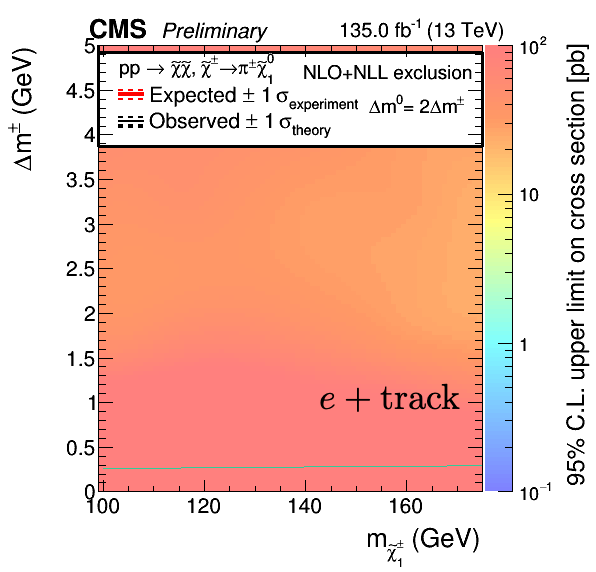
\includegraphics[width=0.48\linewidth]{plots/limits/expected/PureHiggsino_1tElectrons_ExpectedXSEC.png} \,
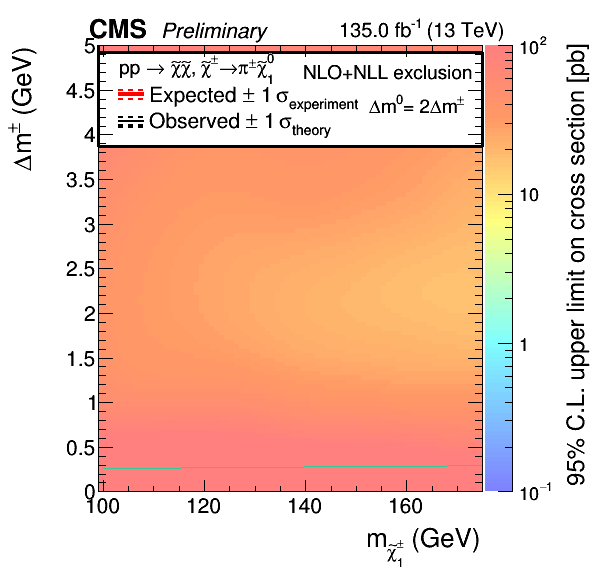
\includegraphics[width=0.48\linewidth]{plots/limits/expected/PureHiggsino_1tMuons_comb_ExpectedXSEC.png} \\

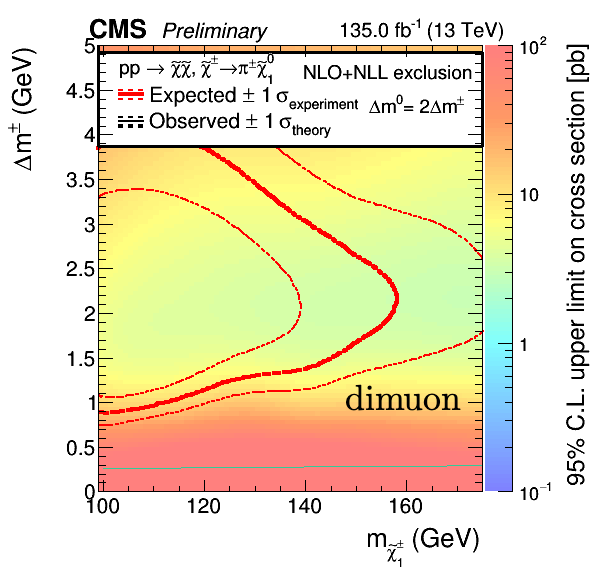
\includegraphics[width=0.48\linewidth]{plots/limits/expected/PureHiggsino_2lMuonsOrth_ExpectedXSEC.png} \,
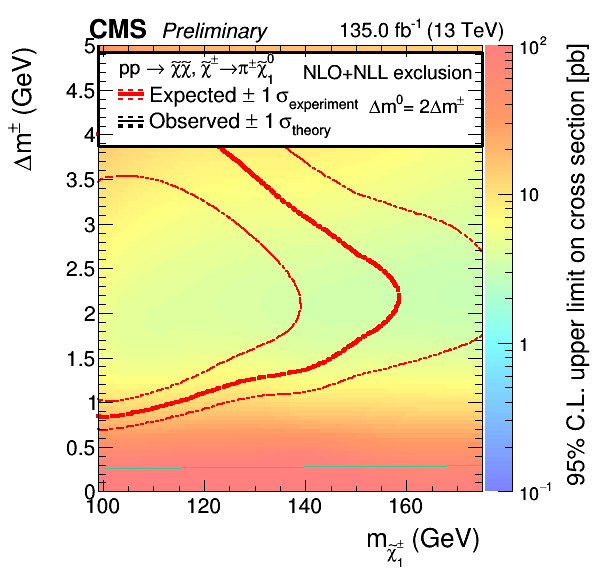
\includegraphics[width=0.48\linewidth]{plots/limits/expected/PureHiggsino_SoftPromptRun2_ExpectedXSEC.png} \\

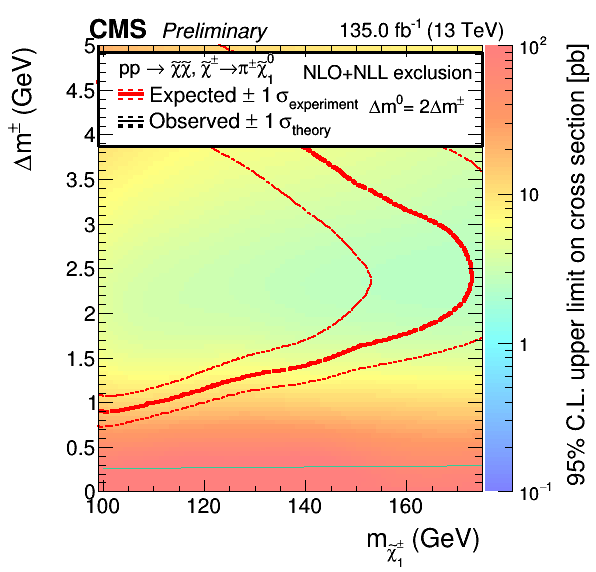
\includegraphics[width=0.48\linewidth]{plots/limits/expected/PureHiggsino_SoftPromptRun2Inc_ExpectedXSEC.png} \\

\caption[Expected limits for full run 2 luminosity]{Expected limits for full run 2 luminosity. Top row shows limits for exclusive track plus electron (muon) on the left (right). The middle row shows limits for the dimuon category (left) and the combined limits for all categories (right). The bottom row shows the combined limits for all categories for the relaxed condition without SOS orthogonality, which was described in Section~\ref{sec:previous-searches}.}
\label{fig:expected_limits}
\end{figure}

\subsection{Partially unblinded results}
\label{sec:unblinded-limits}

In order to perform the unblinding of 10\% of the data, the data-driven background estimation utilizes the full Run 2 luminosity scaled down by 0.1, while the data is taken from 1 out of every 10 events. The data and background predictions are displayed in Figure~\ref{fig:unblinded_results}. The results are presented for the muon plus track category in the first row, the electron plus track category in the middle row, and the dimuon category in the bottom row. Very good agreement is observed in all event categories between the measured data and the background prediction. The largest excess is observed in the right-most bin of the dimuon category in Phase 0. This excess corresponds to $1.4\sigma$ and is interpreted as being in agreement with the SM.

Since the results suggest no deviation from the SM, observed and expected limits are presented in Figure~\ref{fig:observed_limits}. As anticipated, the significantly reduced luminosity approved for unblinding has greatly diminished the expected exclusion. Furthermore, due to the small excess observed in the data compared to the expected count, it was not possible to establish an observed limit.

\begin{figure}[!htb]
\centering
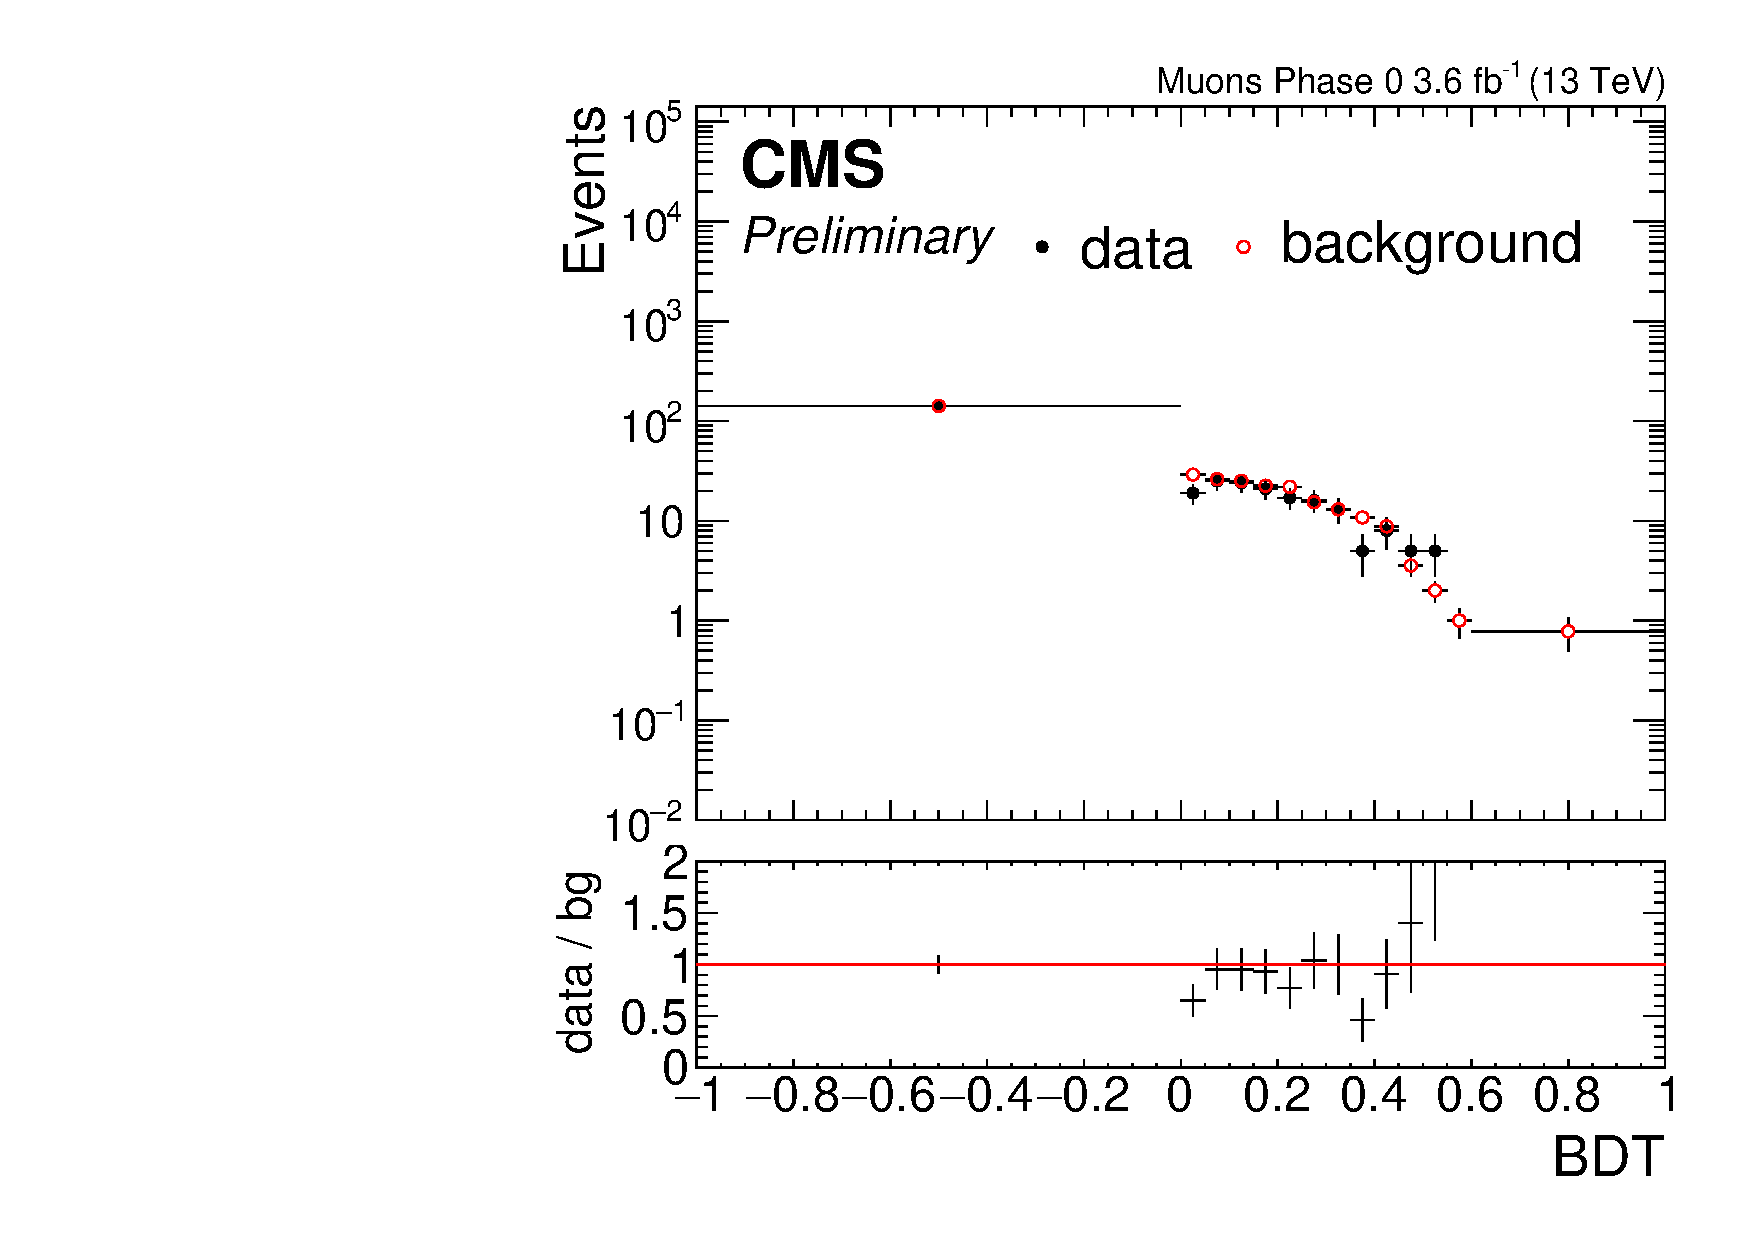
\includegraphics[width=0.48\linewidth]{plots/partial_unblinded_track_muon_sc_comparison/none_exTrack_dilepBDT_binsCorrJetNoMultIso10Dr0.6_log.pdf} \,
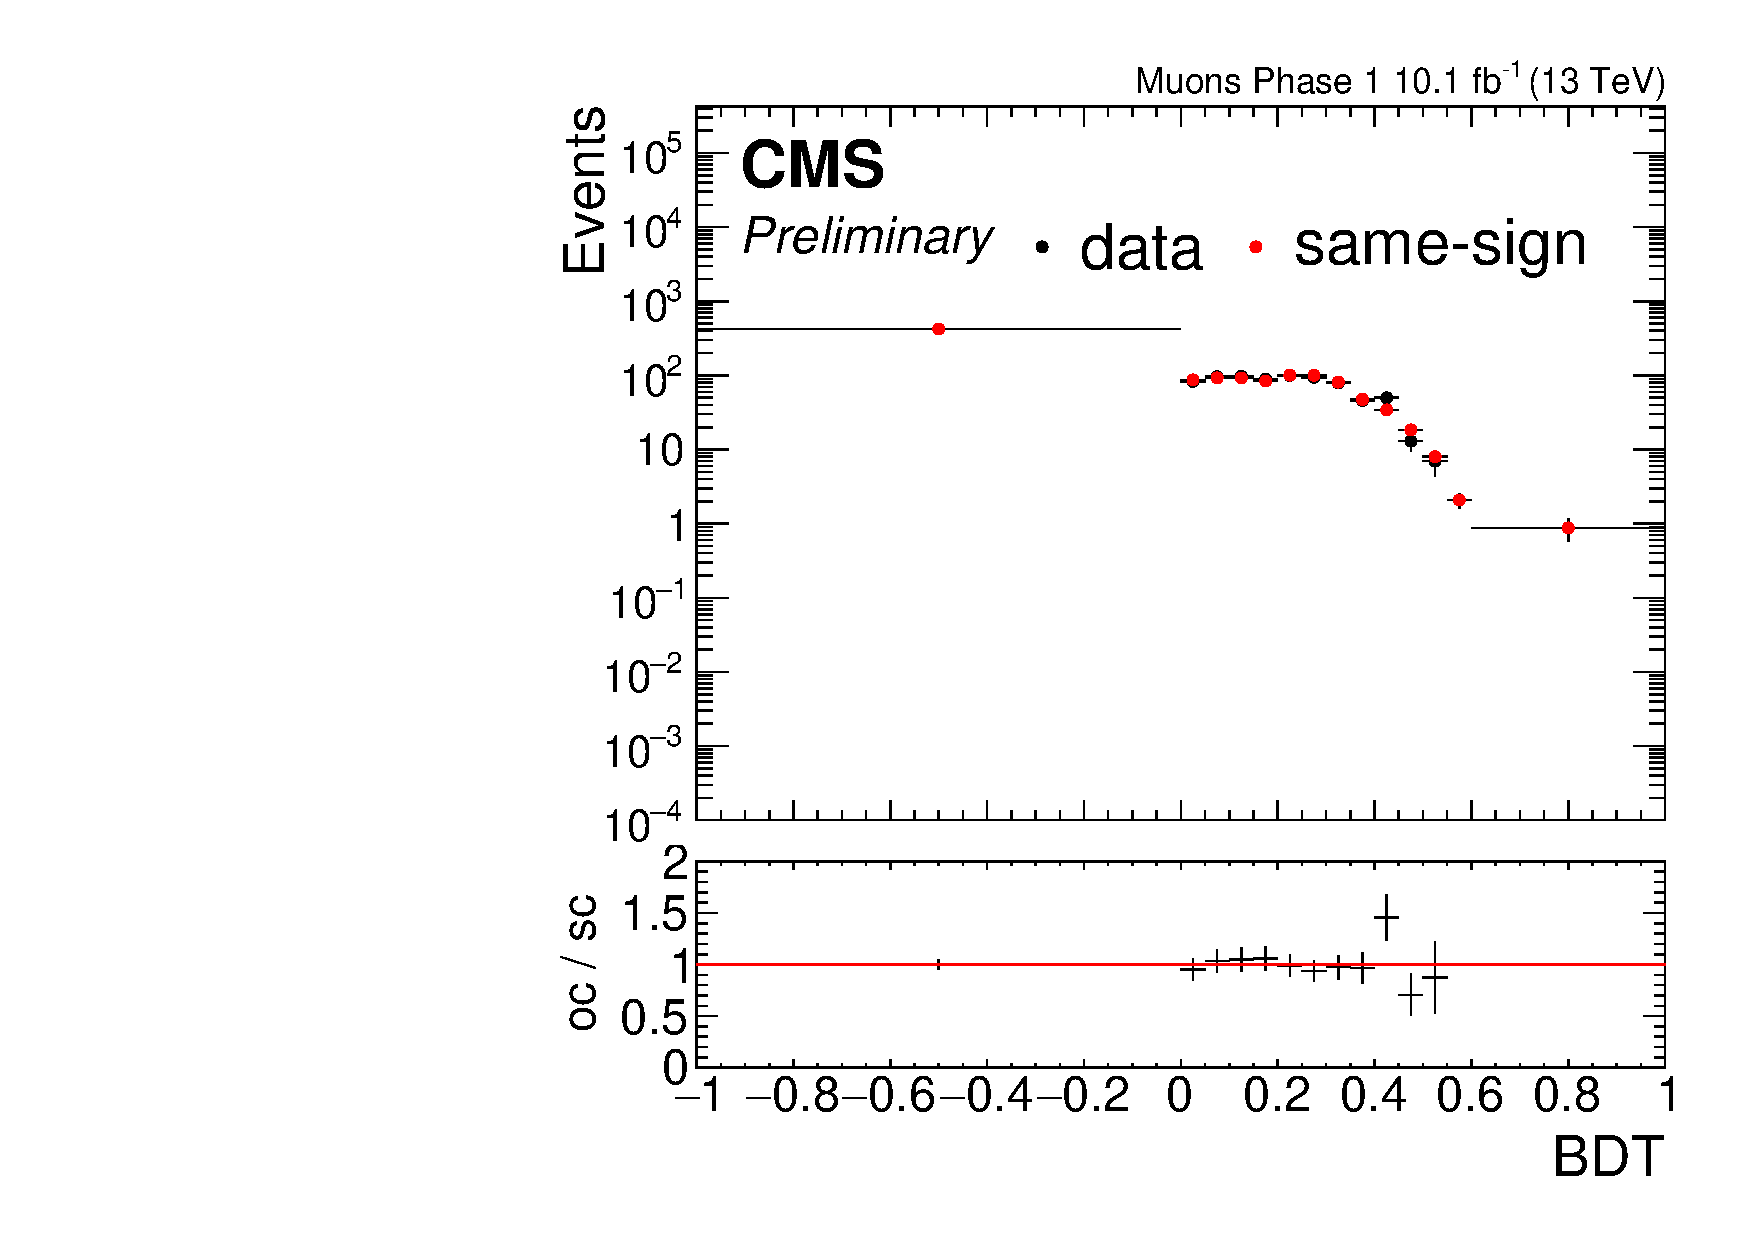
\includegraphics[width=0.48\linewidth]{plots/partial_unblinded_track_muon_sc_comparison_phase1/none_exTrack_dilepBDT_binsCorrJetNoMultIso10Dr0.6_log.pdf} \\

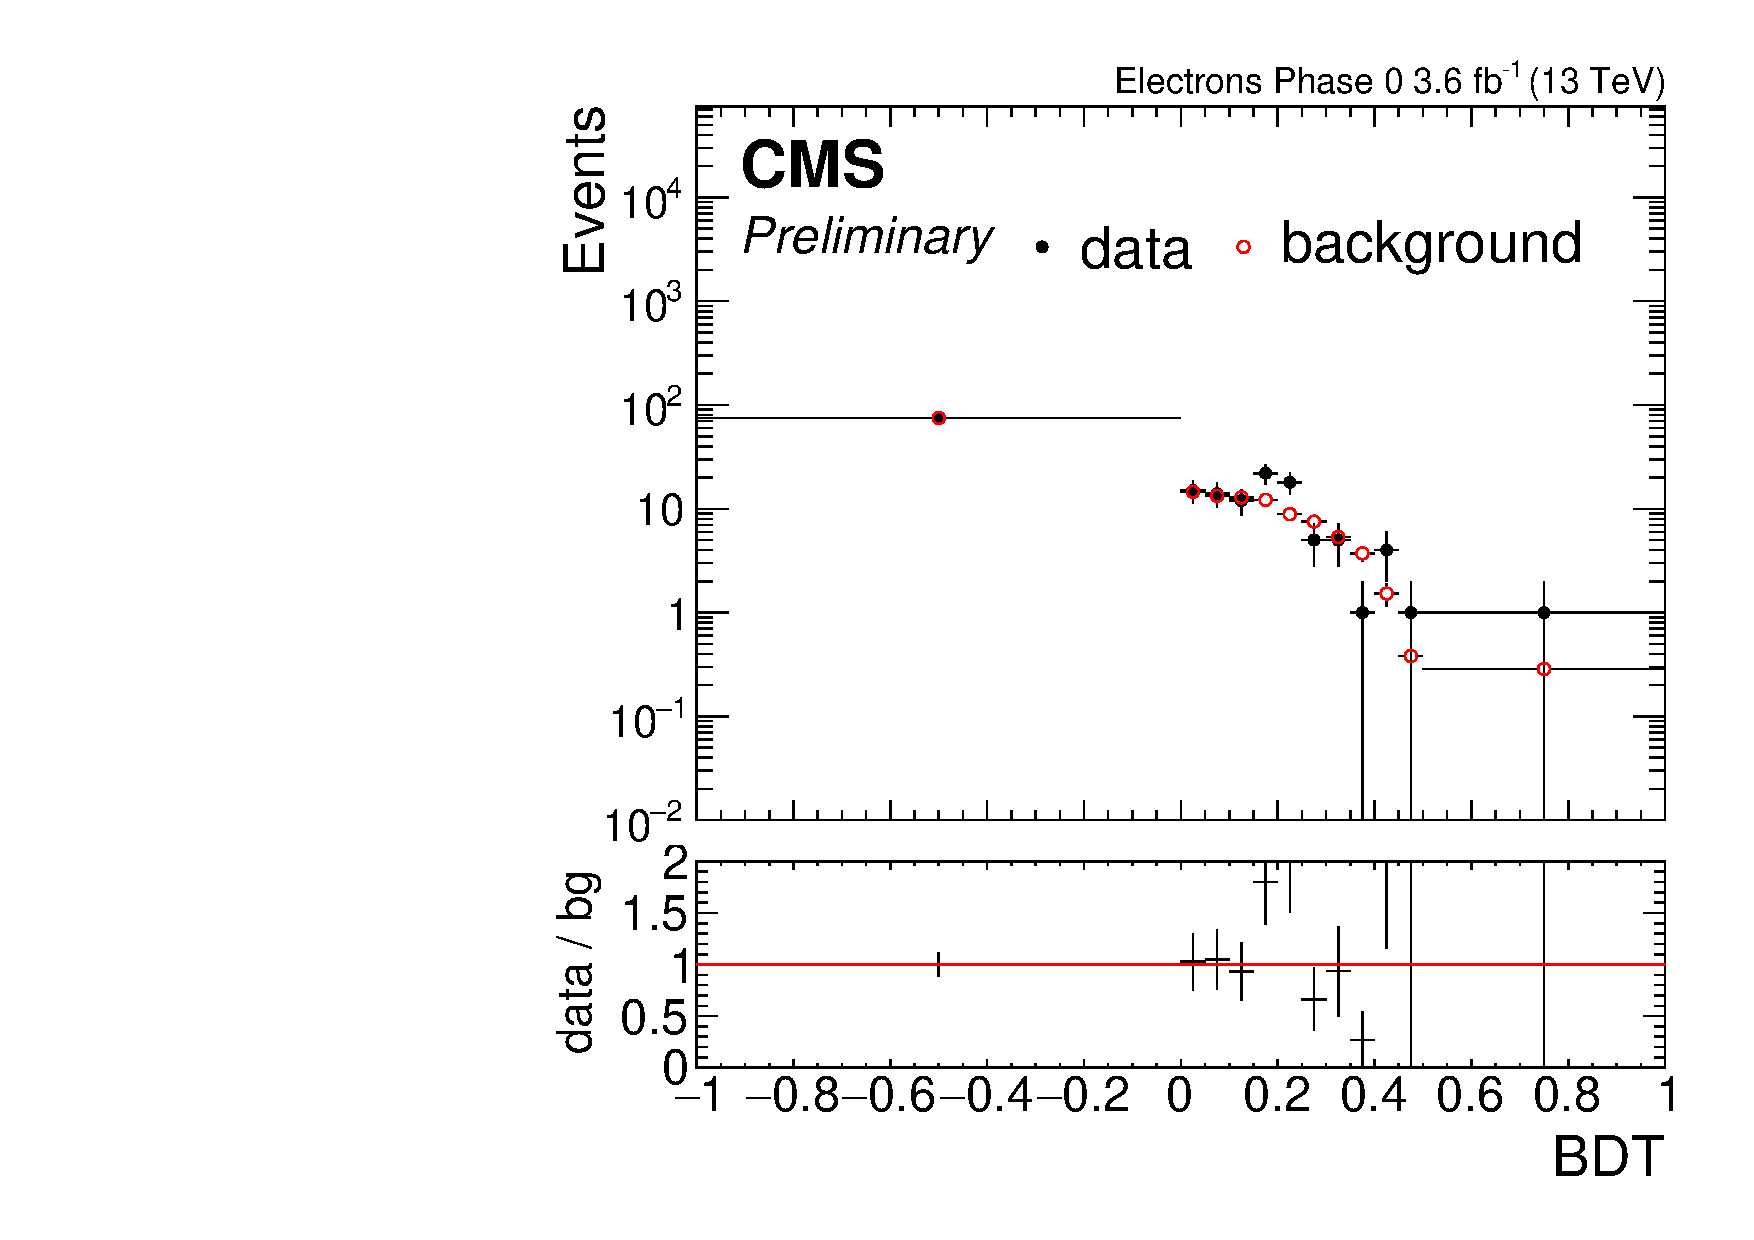
\includegraphics[width=0.48\linewidth]{plots/partial_unblinded_track_electrons_sc_comparison/none_exTrack_dilepBDT_binsCorrJetNoMultIso10Dr0.5_log.pdf} \,
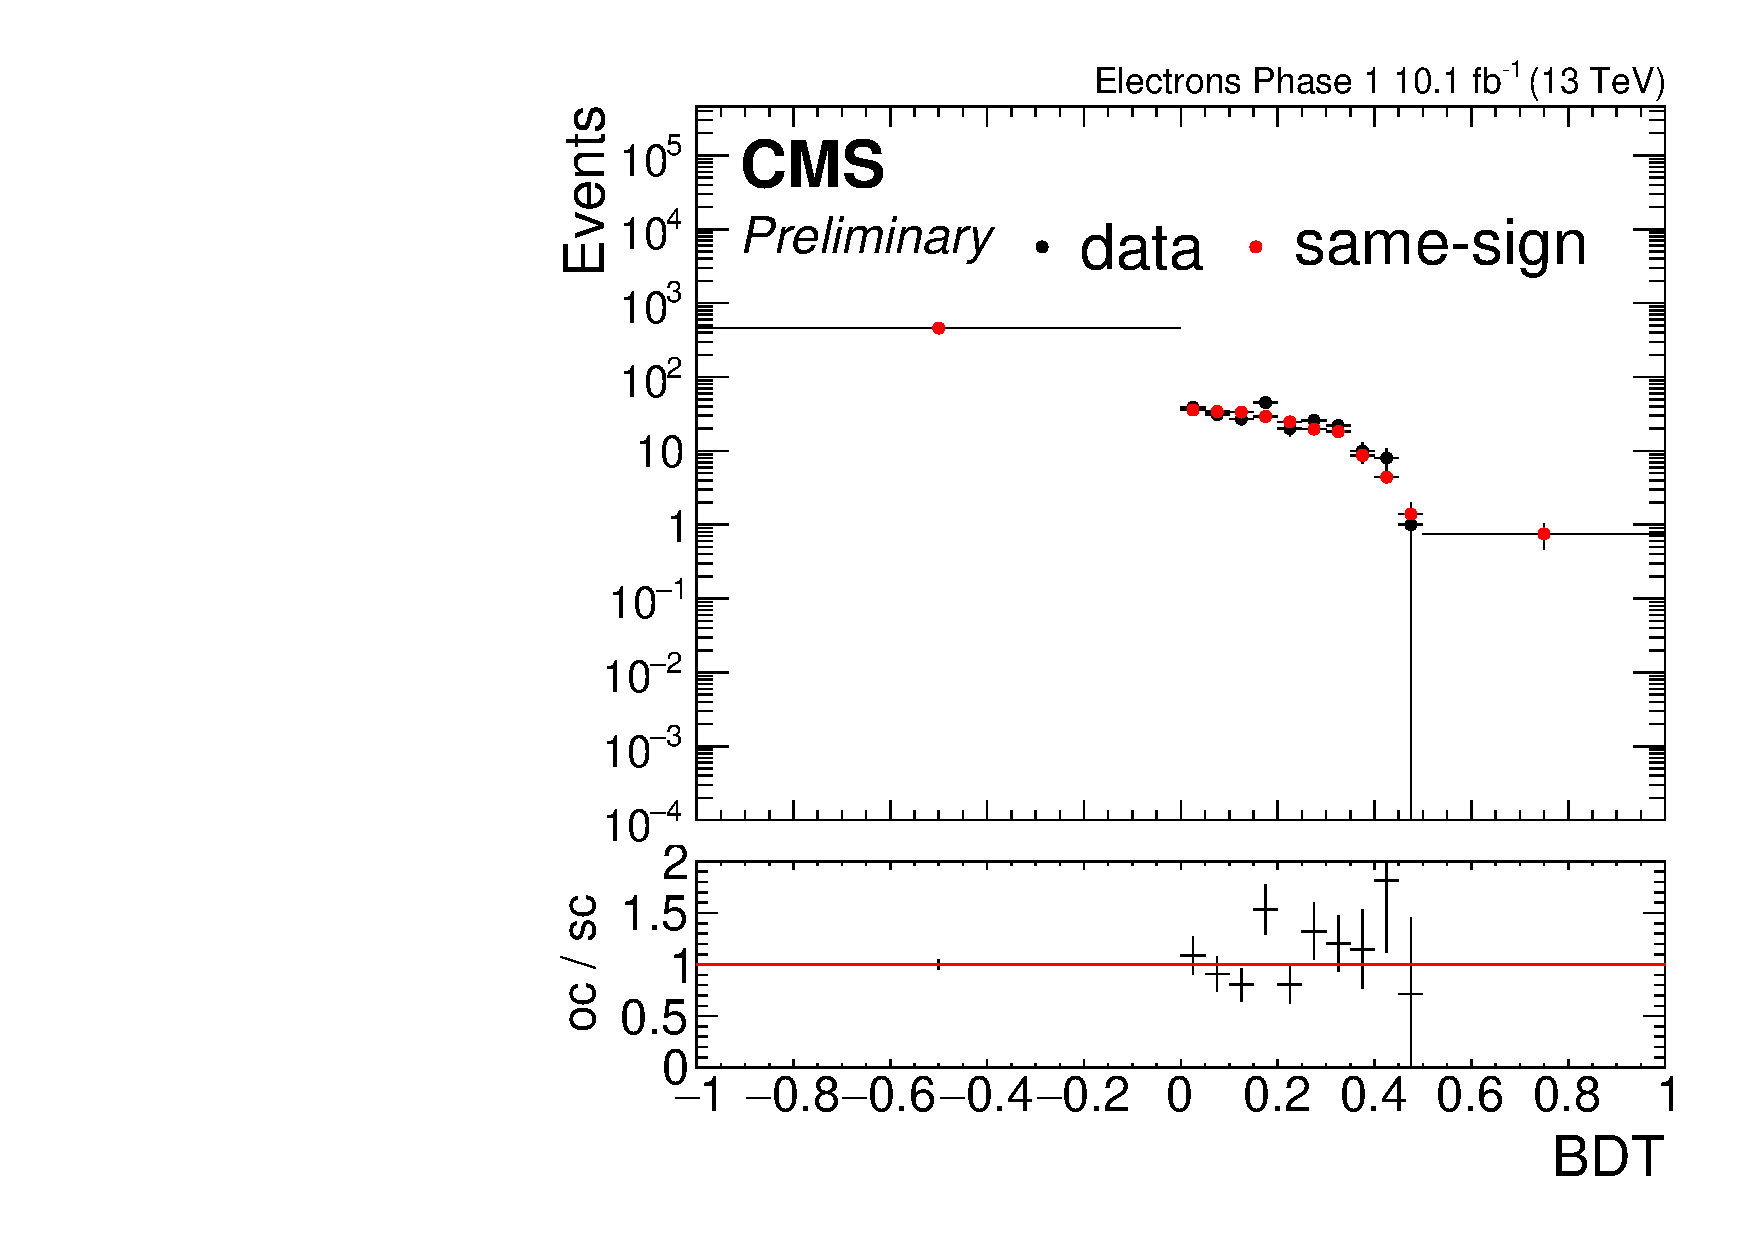
\includegraphics[width=0.48\linewidth]{plots/partial_unblinded_track_electrons_sc_comparison_phase1/none_exTrack_dilepBDT_binsCorrJetNoMultIso10Dr0.5_log.pdf} \\

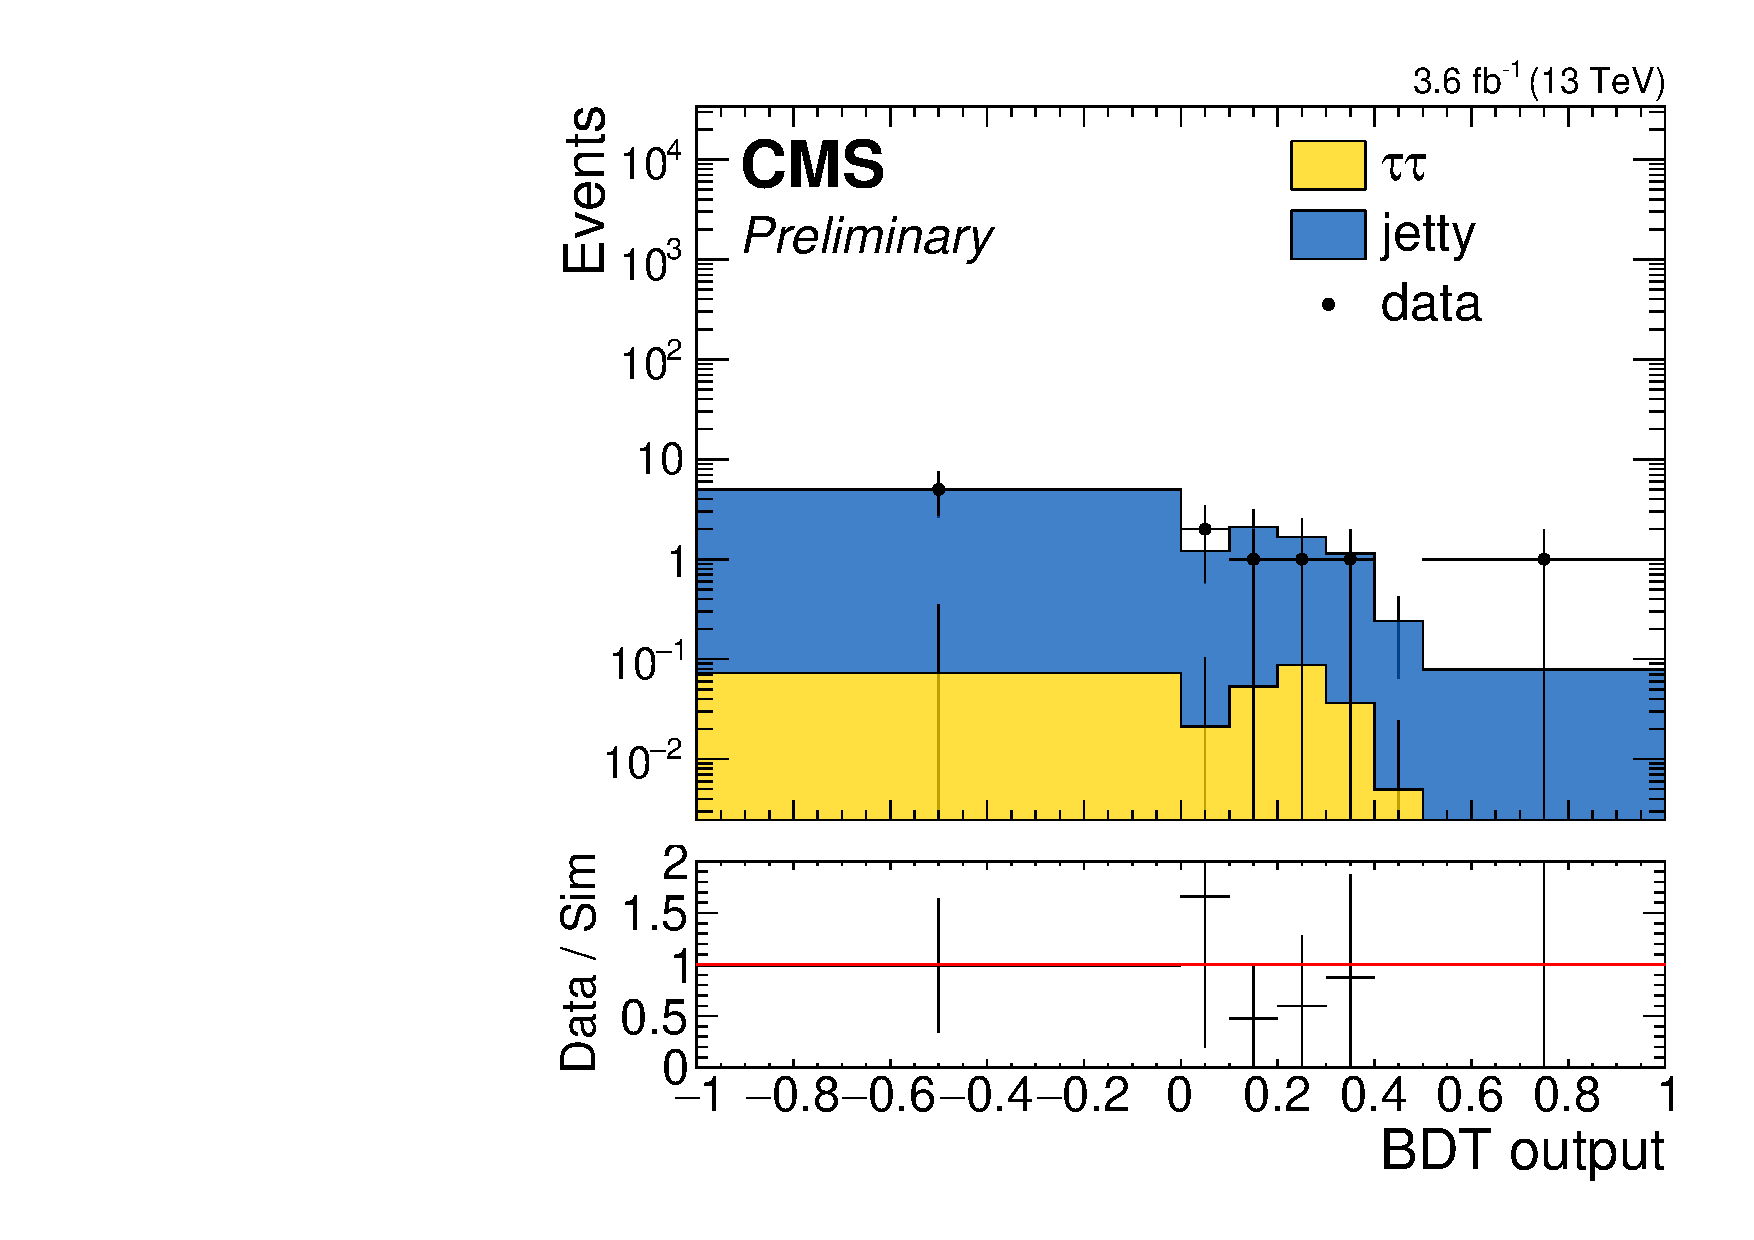
\includegraphics[width=0.48\linewidth]{plots/partial_unblinded_dimuon/sos_final_dilepBDTphase1CorrJetNoMultIso10Dr0.6_log.pdf} \,
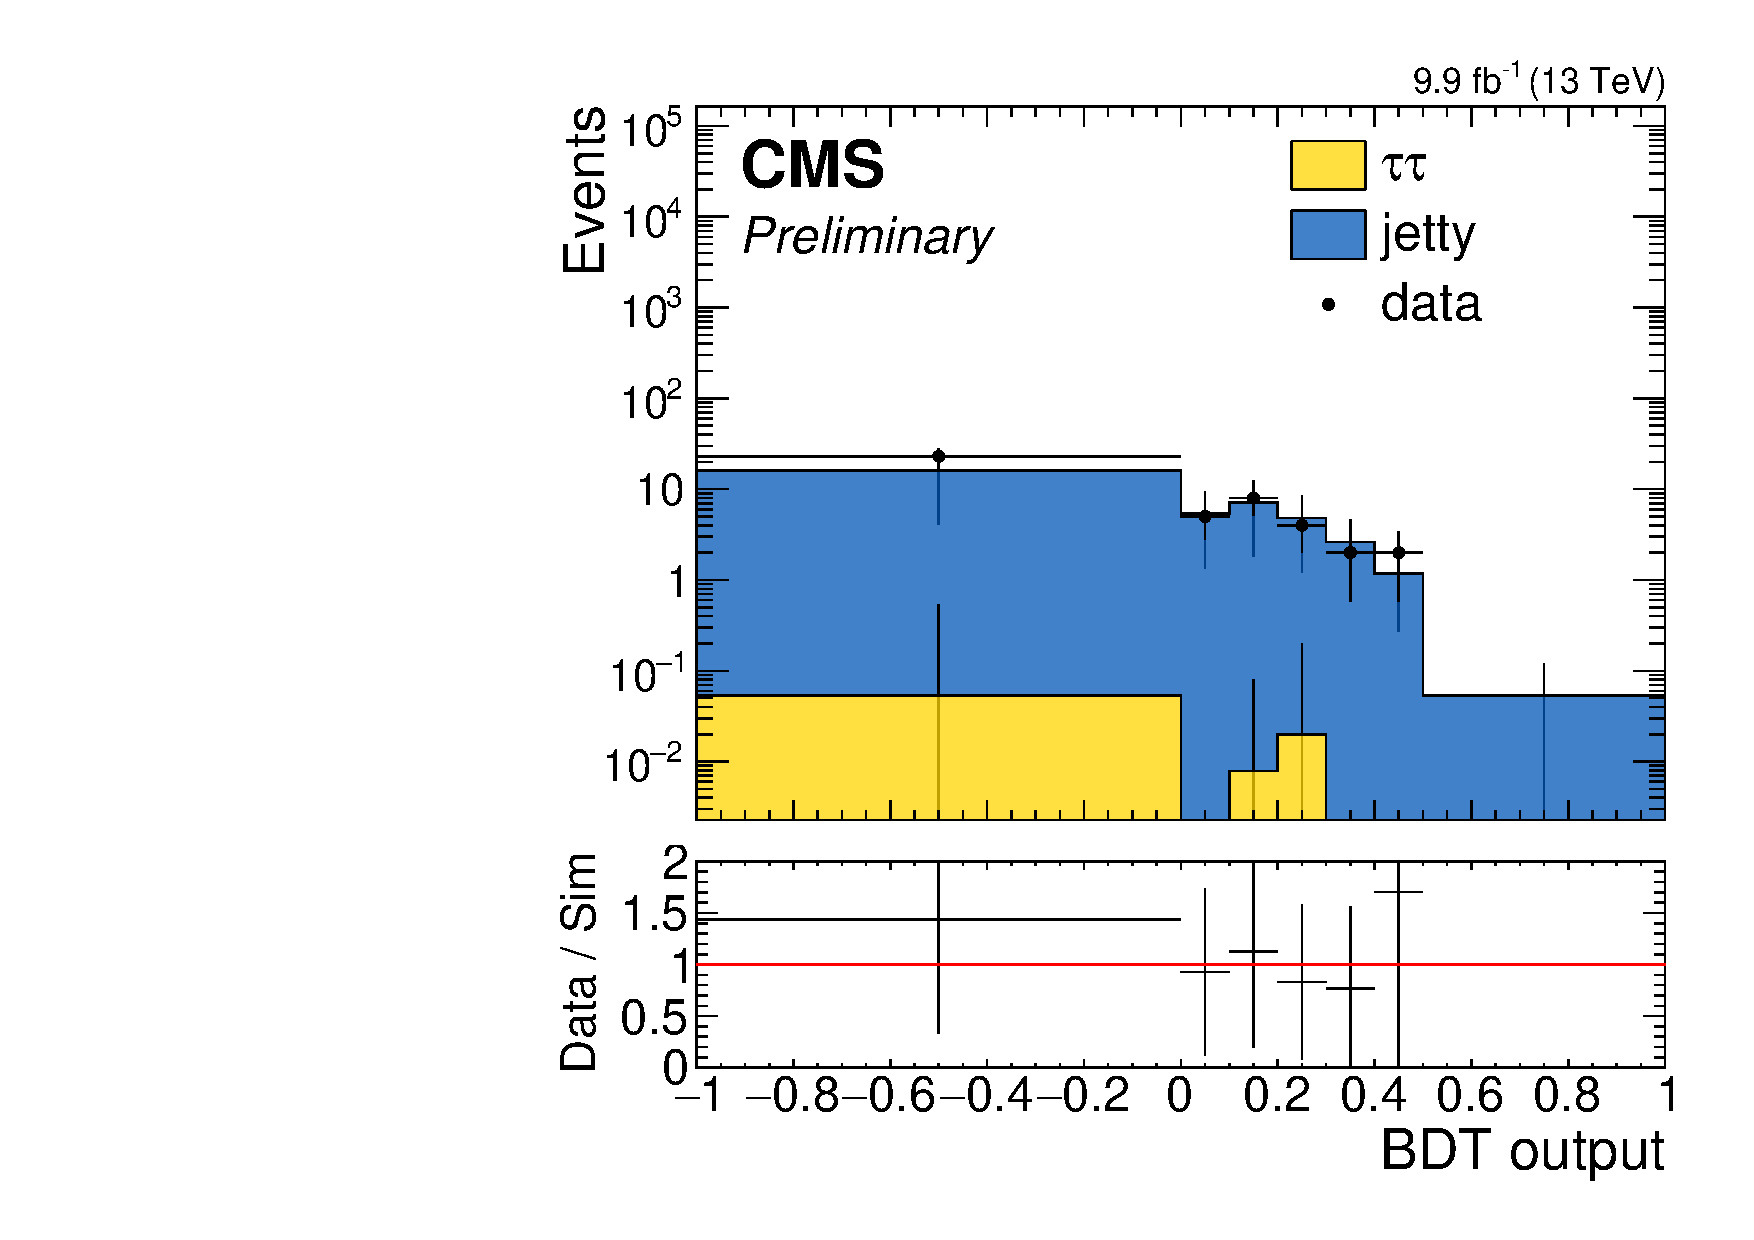
\includegraphics[width=0.48\linewidth]{plots/partial_unblinded_dimuon_phase1/sos_final_dilepBDTCorrJetNoMultIso10Dr0.6_log.pdf} \\

\caption[Partially unblinded results]{Partially unblinded results using 10\% of run 2 luminosity. The top row shows muon plus track category for Phase 0 (left) and Phase 1 (right). The middle row shows the electron plus track category for Phase 0 (left) and Phase 1 (right). Bottom row shows the dimuon category for phase 0 (left) and phase 1 (right).}
\label{fig:unblinded_results}
\end{figure}

\begin{figure}[!htb]
\centering
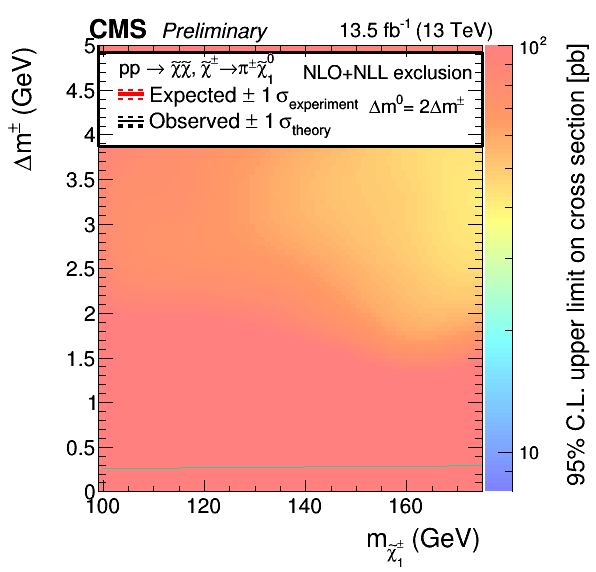
\includegraphics[width=0.48\linewidth]{plots/limits/observed/PureHiggsino_1tElectrons_ObservedXSEC.png} \,
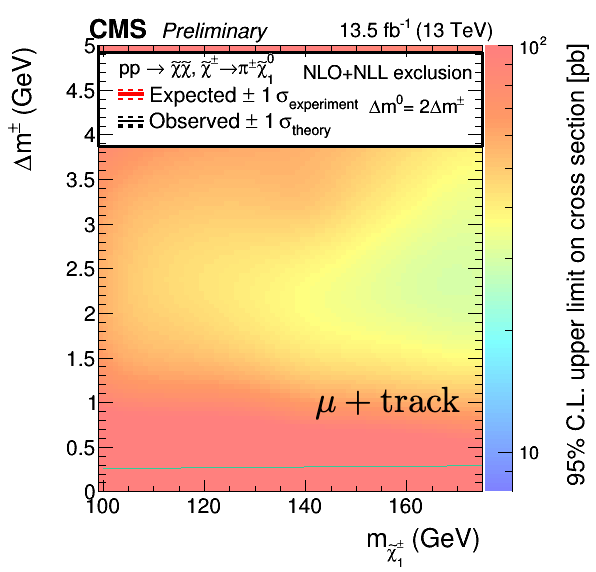
\includegraphics[width=0.48\linewidth]{plots/limits/observed/PureHiggsino_1tMuons_comb_ObservedXSEC.png} \\

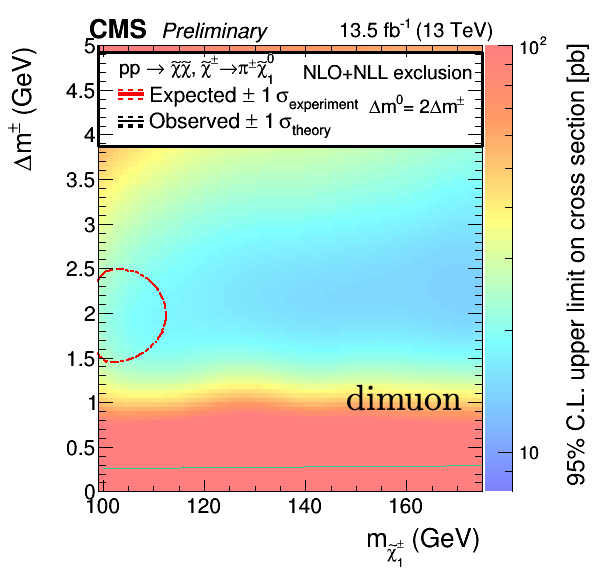
\includegraphics[width=0.48\linewidth]{plots/limits/observed/PureHiggsino_2lMuonsOrth_ObservedXSEC.png} \,
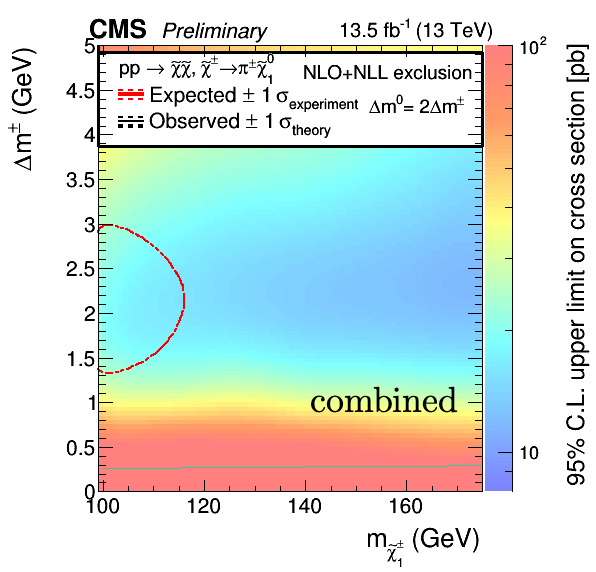
\includegraphics[width=0.48\linewidth]{plots/limits/observed/PureHiggsino_SoftPromptRun2_Observed_XSEC.png} \\

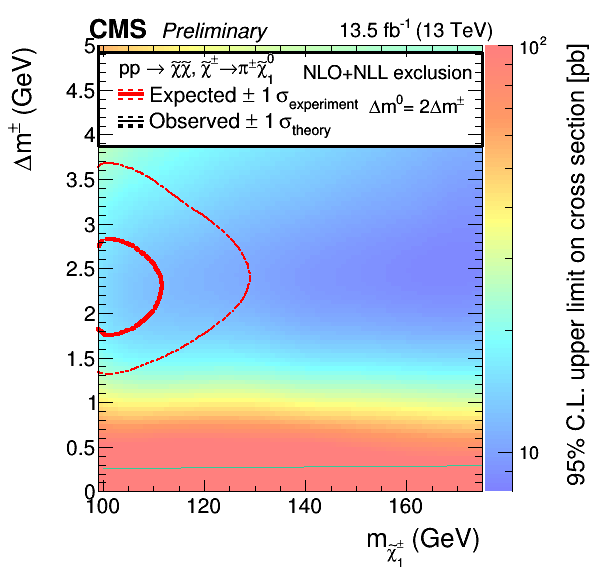
\includegraphics[width=0.48\linewidth]{plots/limits/observed/PureHiggsino_SoftPromptRun2Inc_ObservedXSEC.png} \\

\caption[Expected and observed limits for 10\% luminosity of run 2]{Expected and observed limits for 10\% luminosity of run 2. The top row shows limits for exclusive track plus electron (muon) category on the left (right). The middle row shows limits for the dimuon category (left) and the combined limits for all categories (right). The bottom row shows the combined limits for all categories for the relaxed condition without SOS orthogonality, which was described in Section~\ref{sec:previous-searches}.}
\label{fig:observed_limits}
\end{figure}
